\documentclass[tikz,border=3pt]{standalone}
\usepackage{pgfplots}
\pgfplotsset{compat=1.18}
\begin{document}
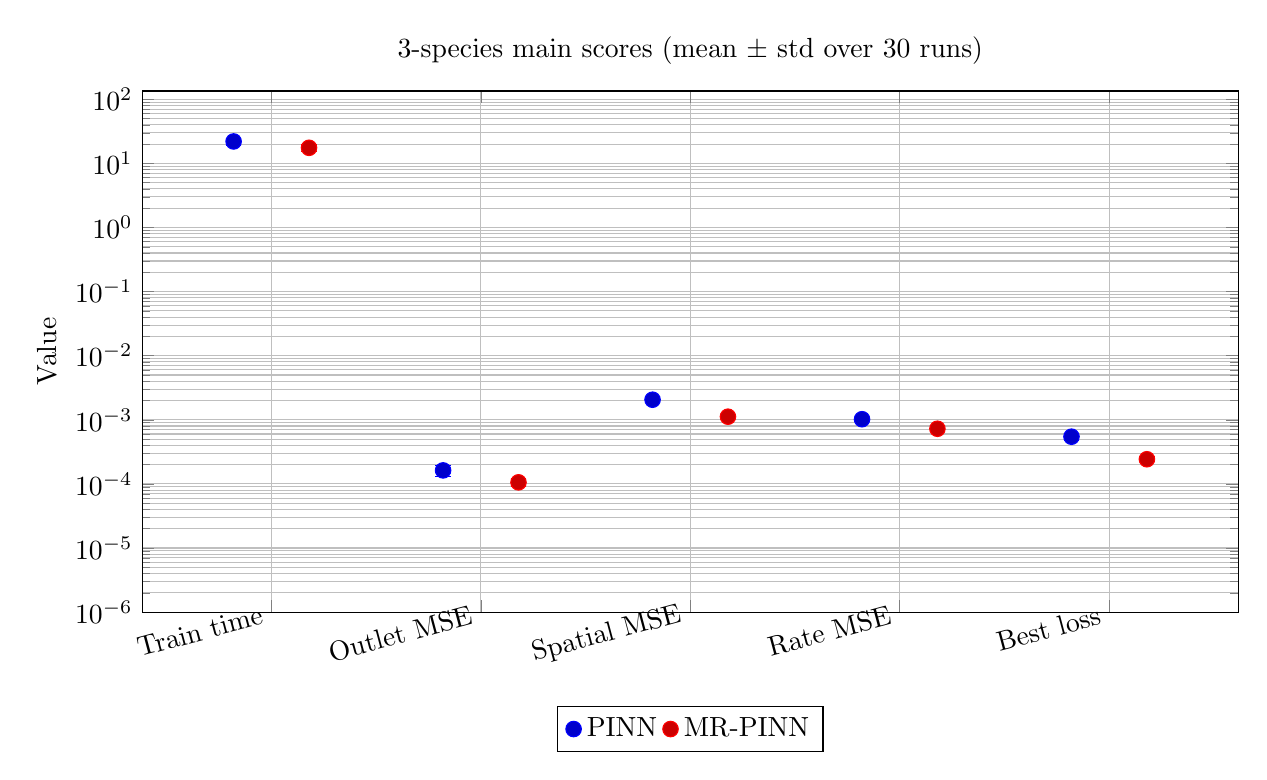
\begin{tikzpicture}
\begin{axis}[
  width=15.5cm,
  height=8.2cm,
  ylabel={Value},
  ymode=log,
  ymin=1e-6,
  grid=both,
  legend style={at={(0.5,-0.18)},anchor=north,legend columns=2},
  xtick={1,2,3,4,5},
  xticklabels={Train time,Outlet MSE,Spatial MSE,Rate MSE,Best loss},
  xticklabel style={rotate=15,anchor=east},
  title={3-species main scores (mean $\pm$ std over 30 runs)},
]
\addplot+[only marks, mark=*, mark size=2.8pt, color=blue, error bars/.cd, y dir=both, y explicit] coordinates {
(0.8200000000000001,22.0224) +- (0,2.6173)
(1.82,1.624304e-04) +- (0,3.077921e-05)
(2.82,0.002058) +- (0,9.799674e-05)
(3.82,0.001021) +- (0,5.488412e-05)
(4.82,5.450375e-04) +- (0,6.222280e-05)
};
\addlegendentry{PINN}
\addplot+[only marks, mark=*, mark size=2.8pt, color=red, error bars/.cd, y dir=both, y explicit] coordinates {
(1.18,17.5358) +- (0,2.0607)
(2.18,1.057256e-04) +- (0,1.372910e-05)
(3.18,0.001118) +- (0,4.779234e-05)
(4.18,7.250416e-04) +- (0,2.332278e-05)
(5.18,2.425059e-04) +- (0,2.202727e-05)
};
\addlegendentry{MR-PINN}
\end{axis}
\end{tikzpicture}
\end{document}